
\documentclass[11pt]{article}
\usepackage[landscape, letterpaper, margin=.75in]{geometry}
\usepackage{graphicx}
\usepackage{amsmath}
\usepackage{multicol}
\begin{document}


    \section{Fractal N = 0}
    \begin{figure}[h!]
      \centering
      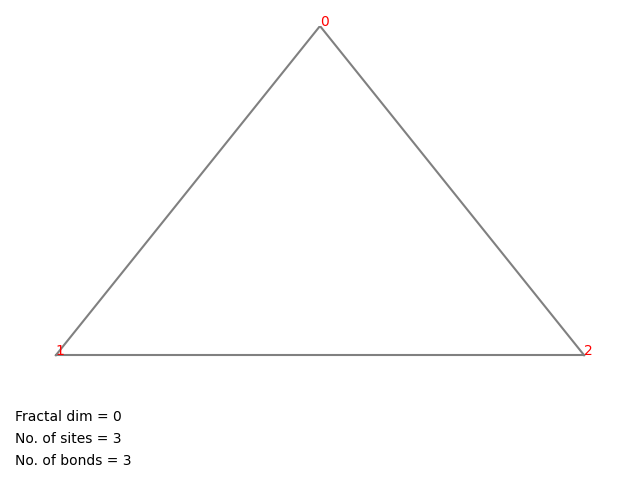
\includegraphics[scale=0.7]{output//N=0//N=0_lattice.png}
      \caption{Lattice}
    \end{figure}
    
    \subsection{Hamoltionian}
    $H=\epsilon \left(\overline{\psi_{0, 0}} \psi_{0, 0} + \overline{\psi_{1, 0}} \psi_{1, 0} + \overline{\psi_{2, 0}} \psi_{2, 0}\right) - t \left(\overline{\psi_{0, 0}} \psi_{1, 0} + \overline{\psi_{0, 0}} \psi_{2, 0} + \overline{\psi_{1, 0}} \psi_{0, 0} + \overline{\psi_{1, 0}} \psi_{2, 0} + \overline{\psi_{2, 0}} \psi_{0, 0} + \overline{\psi_{2, 0}} \psi_{1, 0}\right)$

    \subsection{Matrix}
    $\left[\begin{matrix}\epsilon & - t & - t\\- t & \epsilon & - t\\- t & - t & \epsilon\end{matrix}\right]$

    \subsection{Eigen Values}
    $\left\{ \epsilon - 2 t : 1, \  \epsilon + t : 2\right\}$

    \subsection{Eigen Vectors}
    $\left[ \left( \epsilon - 2 t, \  1, \  \left[ \left[\begin{matrix}1\\1\\1\end{matrix}\right]\right]\right), \  \left( \epsilon + t, \  2, \  \left[ \left[\begin{matrix}-1\\1\\0\end{matrix}\right], \  \left[\begin{matrix}-1\\0\\1\end{matrix}\right]\right]\right)\right]$
    \end{document}